\documentclass{beamer}

\usetheme{Madrid}

\usepackage{iftex}
\ifPDFTeX
  \usepackage{lmodern}
  \usepackage[utf8]{vietnam}
\else
  \usepackage{fontspec}
  \setsansfont{DejaVu Sans}
  \setmainfont{DejaVu Sans}
\fi

\usepackage{xcolor}
\usepackage{colortbl}
\usepackage{graphicx}
\usepackage{amsmath}
\usepackage{booktabs}
\usepackage{tikz}
\usetikzlibrary{arrows.meta,positioning}

\graphicspath{{figures/}{notebooks/}}

\definecolor{accent}{HTML}{B0152F}
\setbeamercolor{frametitle}{bg=white,fg=accent}
\setbeamercolor{structure}{fg=accent}
\setbeamercolor{title}{bg=white,fg=accent}
\setbeamertemplate{navigation symbols}{}
\setbeamertemplate{frametitle}{\vspace{4pt}\textbf{\insertframetitle}\par\vspace{-2pt}}

\newcommand{\hl}[1]{\textbf{\color{accent}#1}}

\title[ASD Screening with ML]{Autism Spectrum Disorder Screening with Machine Learning}
\subtitle{From a leaky baseline to a foundation-model ensemble}
\author[Group --- HUST]{%
  Trần Trung Hiếu \\
  Phạm Song Hào \\
  Nguyễn Đức Hoàng \\
  Vũ Xuân Sơn \\
  Đặng Quốc Vượng}
\institute{Hanoi University of Science and Technology}
\date{\today}

\begin{document}

\begin{frame}
    \titlepage
\end{frame}

\begin{frame}{Outline}
    \tableofcontents
\end{frame}

\section{Problem \& Pipeline}

\begin{frame}{The problem}
\begin{itemize}
    \item Diagnosing ASD is \hl{slow and costly}; early screening helps early support.
    \item The \hl{AQ-10} questionnaire (\texttt{A1}--\texttt{A10}) gives a fast screening score.
    \item A fixed score cut-off is unreliable in the \hl{grey zone} (score 4--6).
\end{itemize}
\vspace{0.3cm}
\textbf{Goal.} Learn from AQ-10 + demographics to flag likely ASD cases ---
\hl{accurately} and \hl{honestly} (no data leakage).
\end{frame}

\begin{frame}{Project pipeline}
\begin{center}
\resizebox{\textwidth}{!}{%
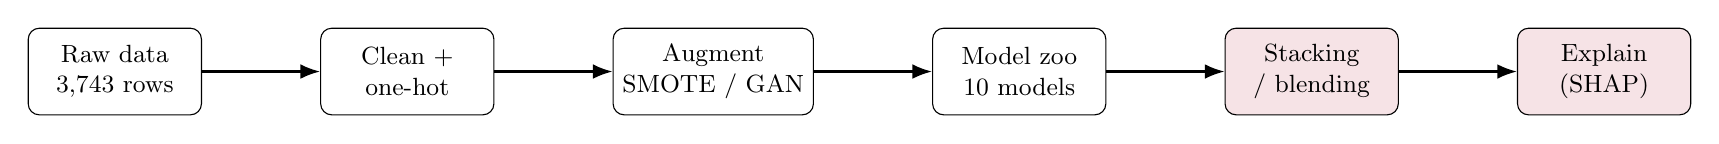
\begin{tikzpicture}[
  node distance=1.5cm,
  box/.style={draw, rounded corners, minimum width=2.2cm, minimum height=1.1cm,
              align=center, font=\small},
  arr/.style={-{Latex[length=2.5mm]}, thick}
]
\node[box] (raw)   {Raw data\\3{,}743 rows};
\node[box, right=of raw]   (clean) {Clean +\\one-hot};
\node[box, right=of clean] (aug)   {Augment\\SMOTE / GAN};
\node[box, right=of aug]   (zoo)   {Model zoo\\10 models};
\node[box, right=of zoo, fill=accent!12] (stack) {Stacking\\/ blending};
\node[box, right=of stack, fill=accent!12] (xai) {Explain\\(SHAP)};
\draw[arr] (raw)--(clean); \draw[arr] (clean)--(aug);
\draw[arr] (aug)--(zoo);   \draw[arr] (zoo)--(stack); \draw[arr] (stack)--(xai);
\end{tikzpicture}%
}
\end{center}
\vspace{0.2cm}
\begin{itemize}
    \item One leakage-free cleaning pipeline feeds \hl{every} model.
    \item Every model uses the \hl{same 5-fold Stratified CV} --- a fair race.
\end{itemize}
\end{frame}

\section{Data \& the leakage pitfall}

\begin{frame}{The raw data --- and its traps}
\begin{columns}
\begin{column}{0.56\textwidth}
\begin{itemize}
    \item 3{,}743 rows, 22 columns, \hl{no missing values}.
    \item \texttt{age} max $= \hl{383}$ $\Rightarrow$ data-entry error.
    \item \texttt{contry\_of\_res}, \texttt{used\_app\_before}: \hl{one value only} (no signal).
    \item \texttt{ethnicity}: duplicates from typos\\(\texttt{White European} vs \texttt{White-European}).
\end{itemize}
\end{column}
\begin{column}{0.44\textwidth}
\begin{center}
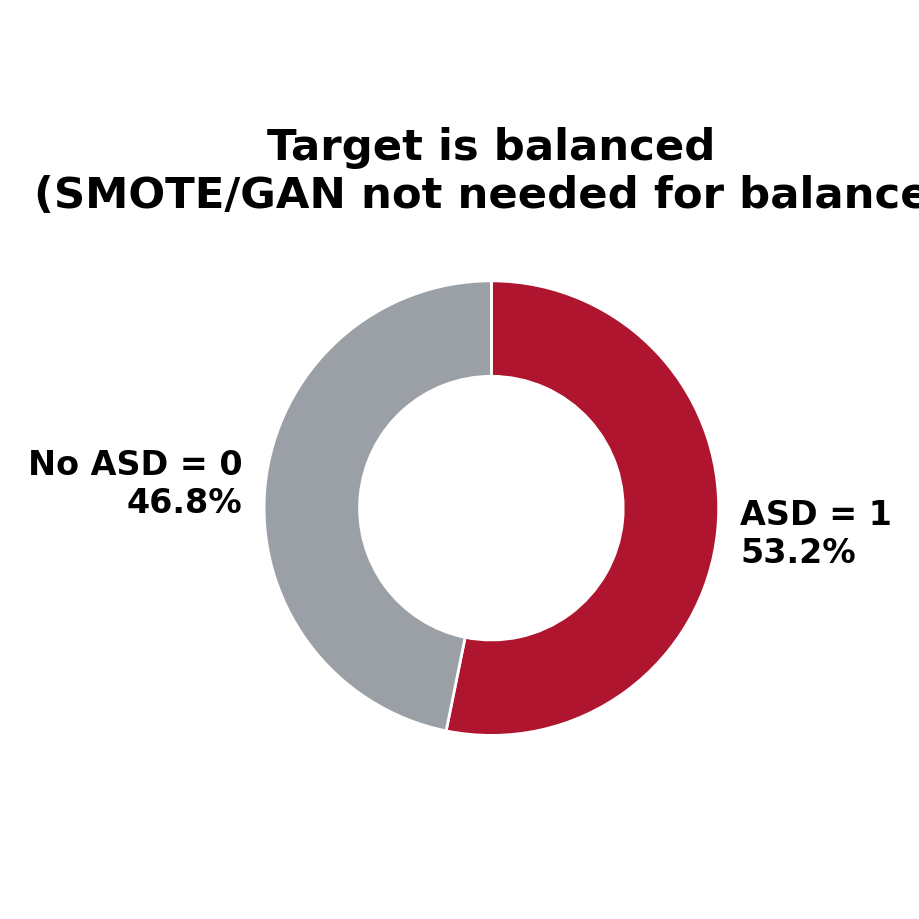
\includegraphics[width=\linewidth]{fig_classbalance.png}
\end{center}
\end{column}
\end{columns}
\vspace{0.1cm}
{\footnotesize Target is balanced (53/47) $\Rightarrow$ SMOTE/GAN are for \emph{robustness}, not for balance.}
\end{frame}

\begin{frame}{Cleaning \& encoding}
\begin{itemize}
    \item Drop zero-variance columns; merge typo categories.
    \item Clip the age outlier to the \hl{median}.
    \item Encode categoricals with \hl{One-Hot} --- safe, no label peeking.
\end{itemize}
\vspace{0.3cm}
{\footnotesize Output: a clean table reused by all later notebooks.}
\end{frame}

\begin{frame}{The target-leakage pitfall}
Early baseline scored a \hl{fake-perfect} ROC-AUC $= 0.9995$. Why?
\[
\text{enc}(c)=\frac{1}{|\{i:x_i=c\}|}\sum_{i:\,x_i=c} y_i
\quad\text{computed on \hl{all} data before CV.}
\]
\begin{itemize}
    \item Encoding a category by its mean \emph{label} leaks the answer $y$.
    \item The model ``sees'' the target through the feature $\Rightarrow$ unreal scores.
    \item \hl{Fix:} compute encodings inside folds, or just use One-Hot.
\end{itemize}
\end{frame}

\begin{frame}{Honest numbers beat perfect numbers}
\begin{center}
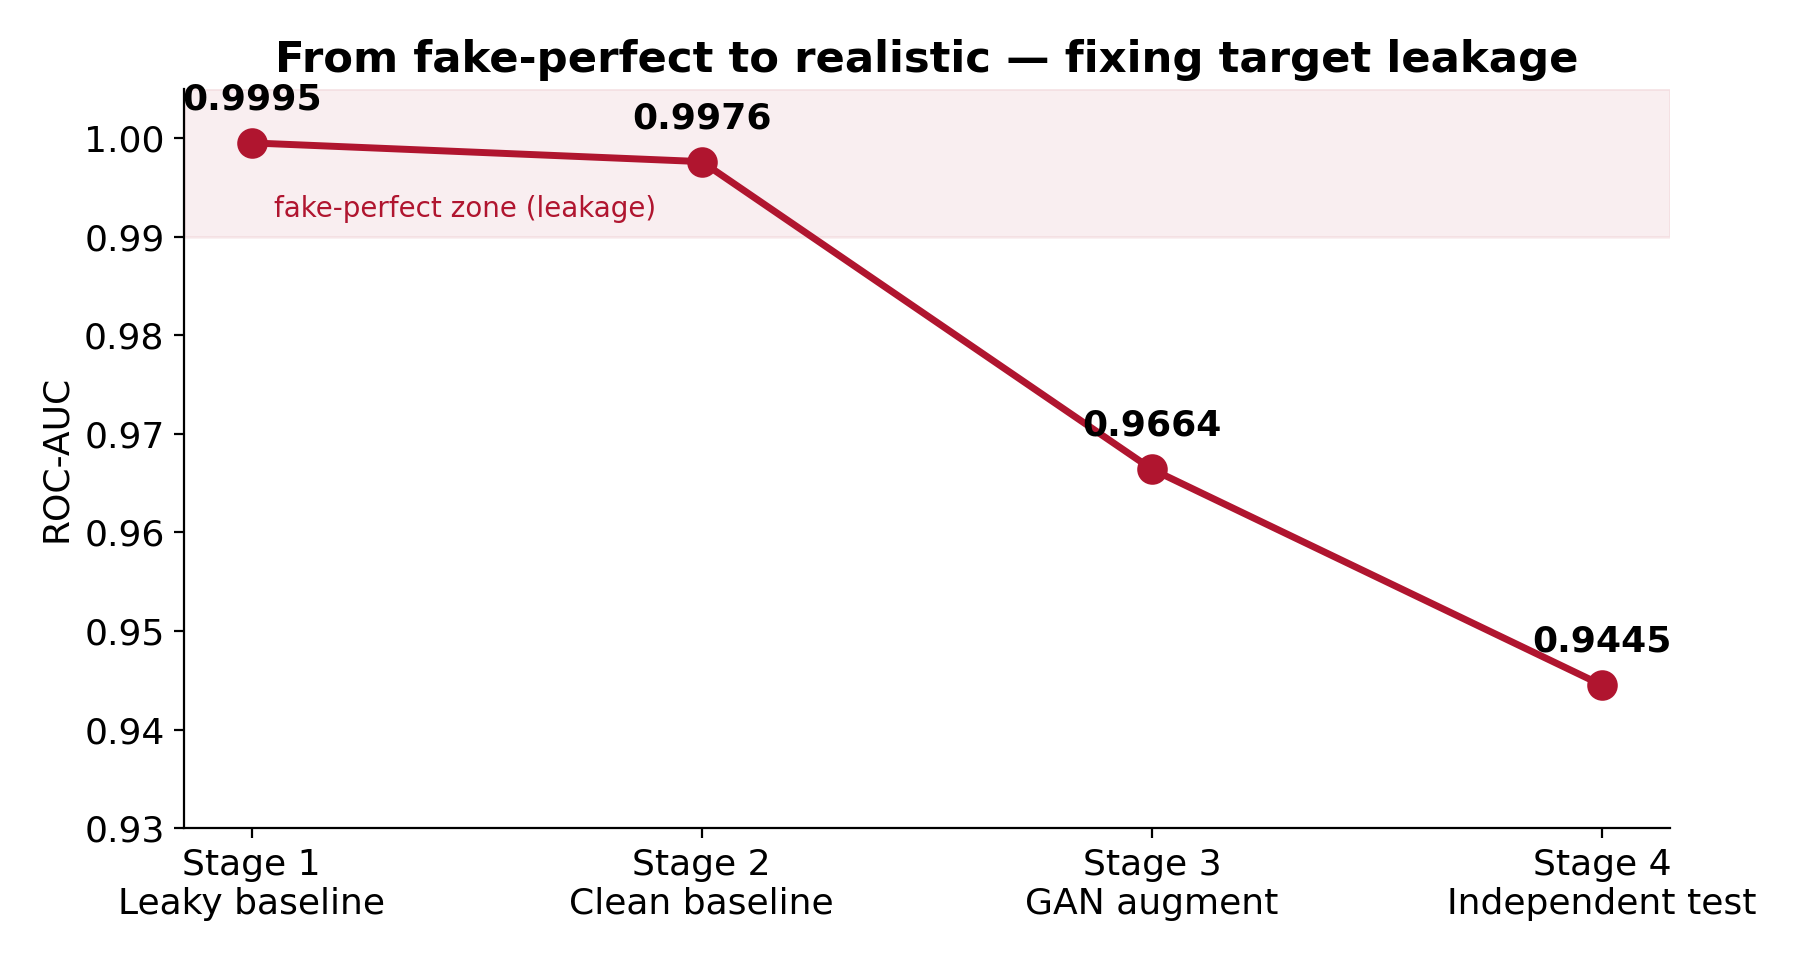
\includegraphics[width=0.86\textwidth]{fig_stages.png}
\end{center}
\vspace{-0.1cm}
{\footnotesize Score \emph{drops} as we remove leakage and add realistic noise ---
this is the model getting \hl{trustworthy}, not weaker.}
\end{frame}

\section{Data generation}

\begin{frame}{SMOTE --- interpolate new samples}
Create a synthetic point between a sample and a neighbour:
\[
x_{\text{new}} = x_i + \lambda\,(x_i^{\text{nn}} - x_i),\qquad \lambda \sim U(0,1).
\]
\begin{itemize}
    \item Fills gaps \emph{between} real points (not blind copies).
    \item Applied \hl{only on the training fold} to avoid leakage.
\end{itemize}
\end{frame}

\begin{frame}{Tabular GAN (PyTorch, from scratch)}
Two networks play a \hl{min--max} game:
\[
\min_G \max_D \; \mathbb{E}_{x}\!\left[\log D(x)\right]
+ \mathbb{E}_{z}\!\left[\log\big(1-D(G(z))\big)\right].
\]
\begin{itemize}
    \item \hl{Generator} $G$: turns noise $z$ into fake patient rows.
    \item \hl{Discriminator} $D$: tells real from fake.
    \item We sampled \hl{+20k} train and \hl{+2k} test rows $\Rightarrow$ harder, more realistic data.
\end{itemize}
\end{frame}

\section{Models}

\begin{frame}{How we compare}
\begin{itemize}
    \item \hl{5-fold Stratified CV} on the unified \hl{23{,}743}-row set.
    \item Headline metrics: \hl{F1-Score} and \hl{ROC-AUC} (threshold-free).
    \item We keep \hl{one leaderboard} and add each new method to it.
\end{itemize}
\end{frame}

\begin{frame}{Baselines --- the classics}
\begin{itemize}
    \item \hl{Logistic Regression} --- linear log-odds: $\log\frac{p}{1-p}=w^{\!\top}x+b$. Simple, interpretable.
    \item \hl{Random Forest} --- average many de-correlated deep trees (bagging) to cut variance.
    \item \hl{AdaBoost} --- add stumps sequentially, re-weighting the samples each one gets wrong.
    \item \hl{XGBoost} --- regularized gradient boosting; our strongest baseline.
\end{itemize}
\vspace{0.2cm}
{\footnotesize These set the bar the modern methods must beat.}
\end{frame}

\begin{frame}{Leaderboard --- baselines}
\footnotesize
Starting point: \hl{XGBoost} leads the four classics.
\vspace{0.25cm}
\begin{center}
\begin{tabular}{lccc}
\toprule
\textbf{Model} & \textbf{Acc} & \textbf{F1} & \textbf{ROC-AUC} \\
\midrule
\rowcolor{accent!18}\textbf{XGBoost} & 0.9162 & 0.9197 & 0.9767 \\
Random Forest & 0.9151 & 0.9191 & 0.9748 \\
AdaBoost & 0.8624 & 0.8656 & 0.9511 \\
Logistic Regression & 0.8643 & 0.8687 & 0.9473 \\
\bottomrule
\end{tabular}
\end{center}
\end{frame}

\begin{frame}{CatBoost --- ordered boosting}
\begin{itemize}
    \item Gradient boosting on \hl{oblivious trees} (same split per level) --- fast and regularized.
    \item Encodes categories with \hl{ordered target statistics}, using only \emph{earlier} rows:
    \[
    \hat{x}_i=\frac{\sum_{j<i}\mathbb{1}[x_j=x_i]\,y_j+a\,p}{\sum_{j<i}\mathbb{1}[x_j=x_i]+a}.
    \]
    \item \hl{Ordered boosting} stops a sample seeing its own label $\Rightarrow$ no prediction shift.
\end{itemize}
\vspace{0.1cm}
{\footnotesize Directly cures the Phase-1 leakage --- and trains in just 15.8s.}
\end{frame}

\begin{frame}{Leaderboard --- + CatBoost}
\footnotesize
CatBoost takes over \hl{\#1}.
\vspace{0.25cm}
\begin{center}
\begin{tabular}{lccc}
\toprule
\textbf{Model} & \textbf{Acc} & \textbf{F1} & \textbf{ROC-AUC} \\
\midrule
\rowcolor{accent!18}\textbf{CatBoost} & 0.9207 & 0.9237 & 0.9794 \\
XGBoost & 0.9162 & 0.9197 & 0.9767 \\
Random Forest & 0.9151 & 0.9191 & 0.9748 \\
AdaBoost & 0.8624 & 0.8656 & 0.9511 \\
Logistic Regression & 0.8643 & 0.8687 & 0.9473 \\
\bottomrule
\end{tabular}
\end{center}
\end{frame}

\begin{frame}{TabM --- one MLP, many members}
\begin{itemize}
    \item A neural net (MLP), but it behaves like \hl{$k$ ensembled MLPs} at $\approx$1$\times$ the cost.
    \item \hl{BatchEnsemble}: one shared matrix $W$ + a rank-1 adapter $(r_k,s_k)$ per member:
    \[
    W_k = W \odot (r_k\,s_k^{\!\top}),\qquad
    \hat{p}=\frac{1}{k}\sum_{m=1}^{k}\mathrm{softmax}\big(f_{W_m}(x)\big).
    \]
    \item Averaging members \hl{reduces variance} (better calibration), adapters keep it cheap.
\end{itemize}
\vspace{0.1cm}
{\footnotesize Top-tier accuracy (AUC 0.9796) but \hl{slow to train} ($\sim$1637s on CPU).}
\end{frame}

\begin{frame}{Leaderboard --- + TabM}
\footnotesize
TabM edges ahead on ROC-AUC.
\vspace{0.25cm}
\begin{center}
\begin{tabular}{lccc}
\toprule
\textbf{Model} & \textbf{Acc} & \textbf{F1} & \textbf{ROC-AUC} \\
\midrule
\rowcolor{accent!18}\textbf{TabM} & 0.9203 & 0.9237 & 0.9796 \\
CatBoost & 0.9207 & 0.9237 & 0.9794 \\
XGBoost & 0.9162 & 0.9197 & 0.9767 \\
Random Forest & 0.9151 & 0.9191 & 0.9748 \\
AdaBoost & 0.8624 & 0.8656 & 0.9511 \\
Logistic Regression & 0.8643 & 0.8687 & 0.9473 \\
\bottomrule
\end{tabular}
\end{center}
\end{frame}

\begin{frame}{LightGBM --- histogram boosting}
\begin{itemize}
    \item Gradient boosting that \hl{bins} continuous features into histograms $\Rightarrow$ fast split search.
    \item \hl{Leaf-wise} (best-first) tree growth + sample/feature bundling for extra speed.
    \item Same additive idea, each tree fitting the negative gradient:
    \[
    F_m(x) = F_{m-1}(x) + \nu\,h_m(x),\qquad h_m \approx -\nabla_F L.
    \]
\end{itemize}
\vspace{0.1cm}
{\footnotesize The \hl{fastest} learner here --- a full 5-fold run in just 1.2s.}
\end{frame}

\begin{frame}{Leaderboard --- + LightGBM}
\footnotesize
Fast and competitive --- lands just behind the leaders.
\vspace{0.25cm}
\begin{center}
\begin{tabular}{lccc}
\toprule
\textbf{Model} & \textbf{Acc} & \textbf{F1} & \textbf{ROC-AUC} \\
\midrule
TabM & 0.9203 & 0.9237 & 0.9796 \\
CatBoost & 0.9207 & 0.9237 & 0.9794 \\
\rowcolor{accent!18}\textbf{LightGBM} & 0.9187 & 0.9220 & 0.9780 \\
XGBoost & 0.9162 & 0.9197 & 0.9767 \\
Random Forest & 0.9151 & 0.9191 & 0.9748 \\
AdaBoost & 0.8624 & 0.8656 & 0.9511 \\
Logistic Regression & 0.8643 & 0.8687 & 0.9473 \\
\bottomrule
\end{tabular}
\end{center}
\end{frame}

\begin{frame}{TabPFN --- a tabular foundation model}
\begin{itemize}
    \item A \hl{transformer} pre-trained \emph{once} on millions of synthetic tables.
    \item At use time: feed the training rows + a test row as context, predict in \hl{one forward pass}
    --- \hl{no gradient training, no tuning}:
    \[
    p\big(y \mid x,\, \mathcal{D}_{\text{train}}\big)\;\approx\;\text{single in-context inference}.
    \]
    \item Learns a prior over datasets $\Rightarrow$ approximates the Bayesian posterior predictive.
\end{itemize}
\vspace{0.1cm}
{\footnotesize \hl{Best single model} (F1 0.9275, AUC 0.9810) in $\sim$42s, straight out of the box.}
\end{frame}

\begin{frame}{Leaderboard --- + TabPFN}
\footnotesize
\hl{TabPFN jumps straight to \#1} --- with no tuning at all.
\vspace{0.25cm}
\begin{center}
\begin{tabular}{lccc}
\toprule
\textbf{Model} & \textbf{Acc} & \textbf{F1} & \textbf{ROC-AUC} \\
\midrule
\rowcolor{accent!18}\textbf{TabPFN} & 0.9241 & 0.9275 & 0.9810 \\
TabM & 0.9203 & 0.9237 & 0.9796 \\
CatBoost & 0.9207 & 0.9237 & 0.9794 \\
LightGBM & 0.9187 & 0.9220 & 0.9780 \\
XGBoost & 0.9162 & 0.9197 & 0.9767 \\
Random Forest & 0.9151 & 0.9191 & 0.9748 \\
AdaBoost & 0.8624 & 0.8656 & 0.9511 \\
Logistic Regression & 0.8643 & 0.8687 & 0.9473 \\
\bottomrule
\end{tabular}
\end{center}
\end{frame}

\begin{frame}{Stacking \& blending}
\begin{itemize}
    \item Train base models with CV, keep their \hl{out-of-fold (OOF)} predictions (leakage-free).
    \item \hl{Blending} --- average the probabilities: $\;\hat{p}=\tfrac{1}{M}\sum_m p_m(x)$.
    \item \hl{Stacking} --- a logistic-regression meta-learner over those predictions:
    \[
    \hat{p}=\sigma\!\Big(\sum_m w_m\,p_m(x)+b\Big).
    \]
    \item Diverse models' errors partly cancel $\Rightarrow$ \hl{steadier} than any single model.
\end{itemize}
\vspace{0.1cm}
{\footnotesize Base learners: TabPFN + CatBoost + LightGBM + XGBoost.}
\end{frame}

\begin{frame}{Leaderboard --- + Stacking \& Blending}
\scriptsize
Ensembles fill the podium just under TabPFN.
\vspace{0.15cm}
\begin{center}
\begin{tabular}{lccc}
\toprule
\textbf{Model} & \textbf{Acc} & \textbf{F1} & \textbf{ROC-AUC} \\
\midrule
TabPFN & 0.9241 & 0.9275 & 0.9810 \\
\rowcolor{accent!18}\textbf{Stacking (LR)} & 0.9232 & 0.9266 & 0.9807 \\
\rowcolor{accent!18}\textbf{Blend (avg 4)} & 0.9226 & 0.9258 & 0.9799 \\
TabM & 0.9203 & 0.9237 & 0.9796 \\
CatBoost & 0.9207 & 0.9237 & 0.9794 \\
LightGBM & 0.9187 & 0.9220 & 0.9780 \\
XGBoost & 0.9162 & 0.9197 & 0.9767 \\
Random Forest & 0.9151 & 0.9191 & 0.9748 \\
AdaBoost & 0.8624 & 0.8656 & 0.9511 \\
Logistic Regression & 0.8643 & 0.8687 & 0.9473 \\
\bottomrule
\end{tabular}
\end{center}
\end{frame}

\section{Results}

\begin{frame}{Final leaderboard}
\begin{center}
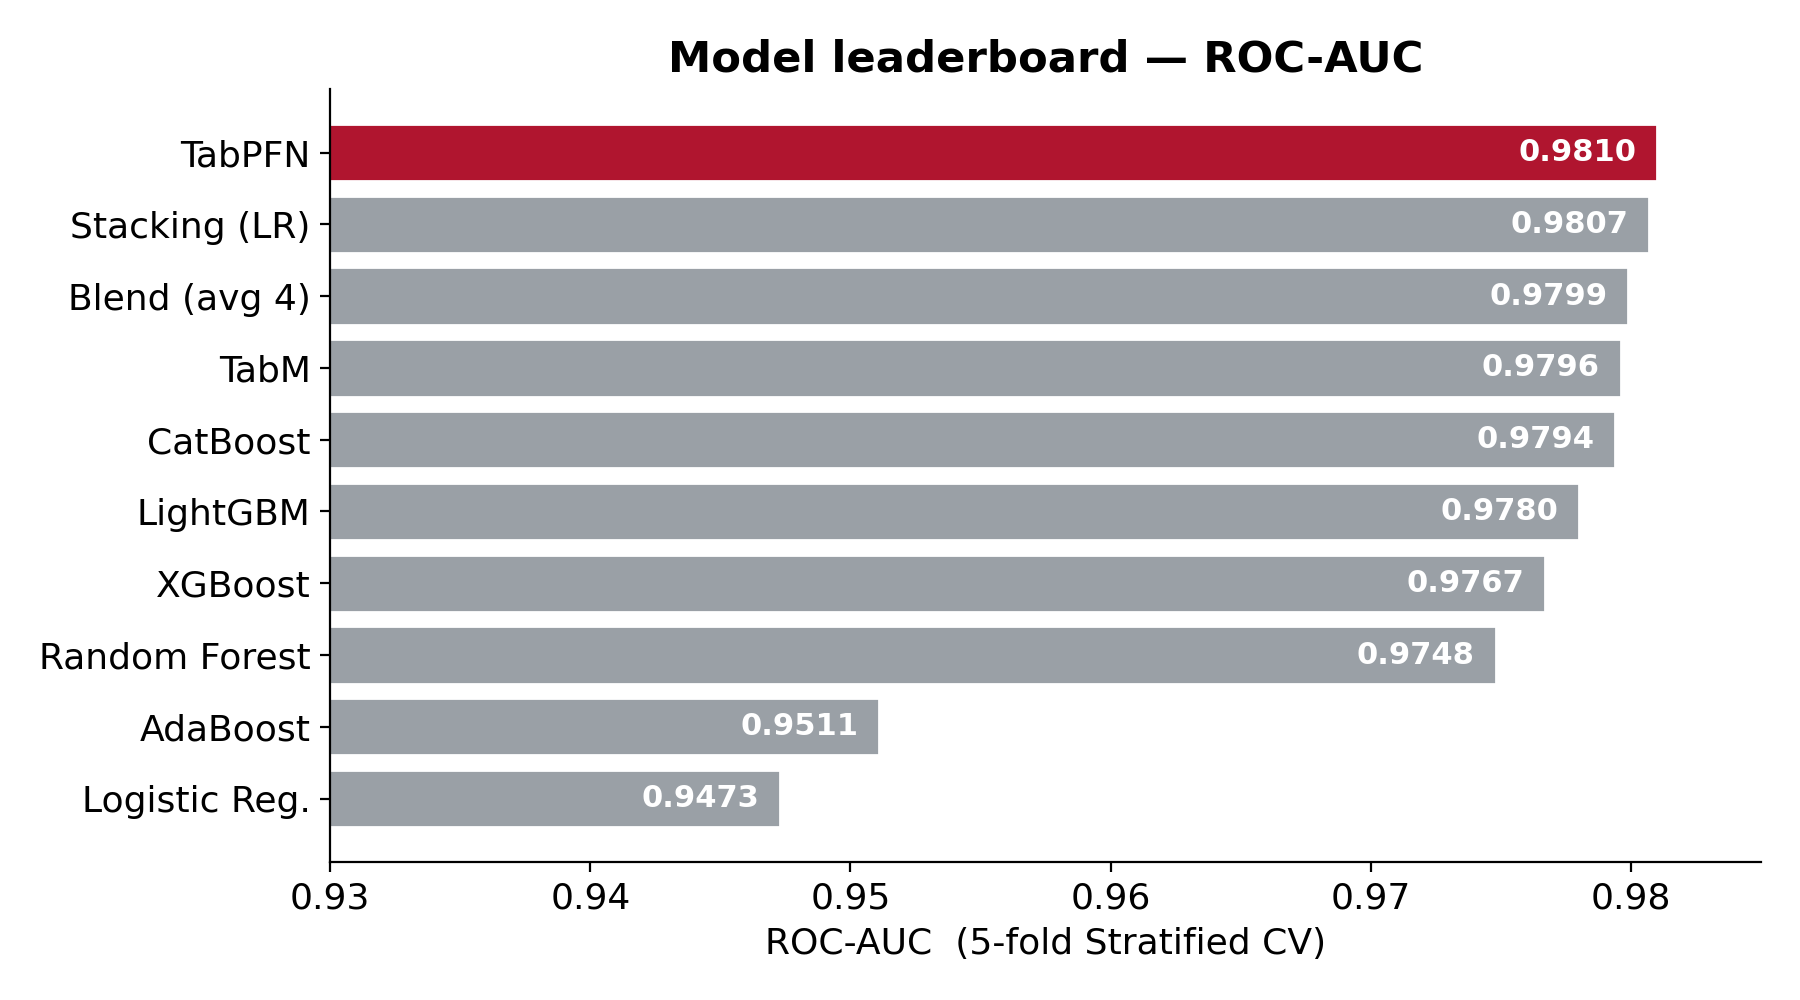
\includegraphics[width=0.9\textwidth]{fig_leaderboard_auc.png}
\end{center}
\vspace{-0.15cm}
{\footnotesize From \hl{LogReg 0.947} to \hl{TabPFN 0.981} ROC-AUC. Top-3 = foundation model
+ ensembles; a zero-tuning model wins.}
\end{frame}

\begin{frame}{Accuracy vs. cost}
\begin{columns}
\begin{column}{0.6\textwidth}
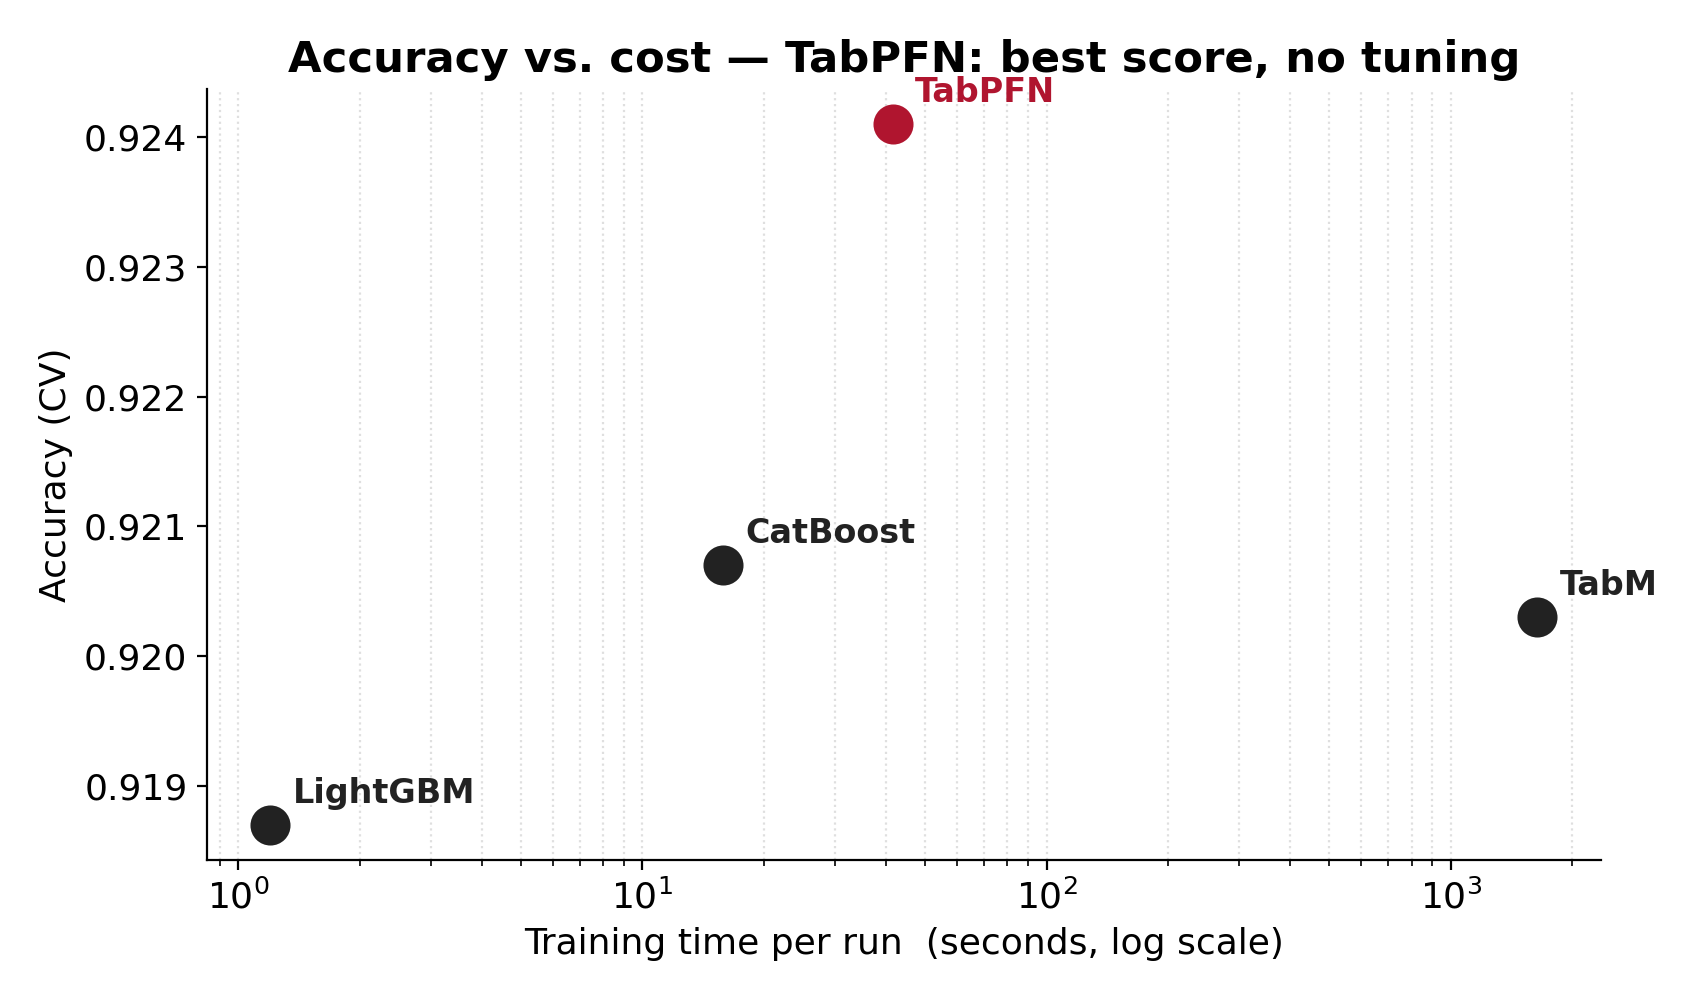
\includegraphics[width=\linewidth]{fig_acc_vs_time.png}
\end{column}
\begin{column}{0.4\textwidth}
\begin{itemize}\small
    \item \hl{LightGBM}: 1.2s, very strong value.
    \item \hl{TabPFN}: best score, $\sim$42s, no tuning.
    \item \hl{TabM}: 1637s --- accuracy at a steep cost.
\end{itemize}
\end{column}
\end{columns}
\end{frame}

\begin{frame}{Explainable AI --- which features matter (global)}
\begin{columns}
\begin{column}{0.55\textwidth}
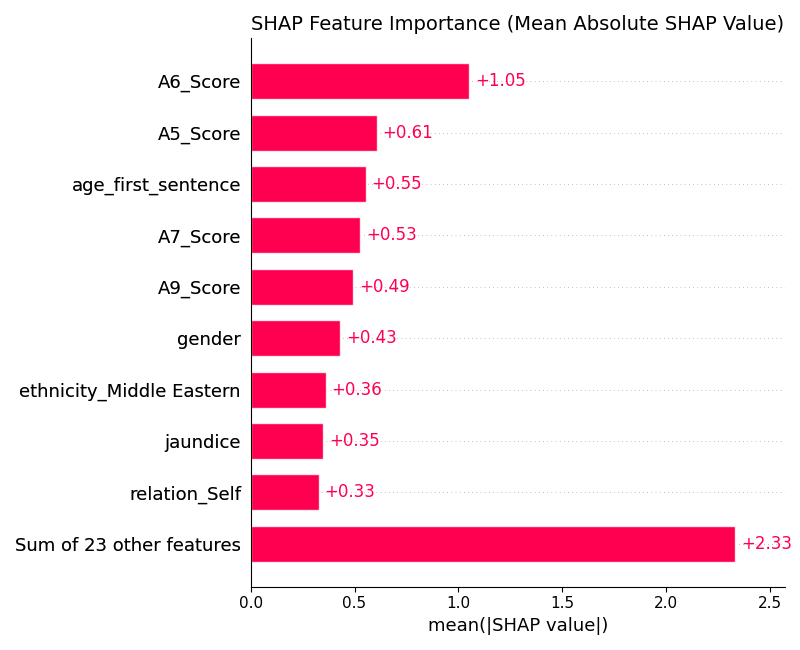
\includegraphics[width=\linewidth]{shap_bar_plot.png}
\end{column}
\begin{column}{0.45\textwidth}
\small
SHAP value = a feature's fair contribution (Shapley value):
\[
\phi_i\!=\!\!\!\sum_{S\subseteq F\setminus\{i\}}\!\!\!
\frac{|S|!\,(|F|\!-\!|S|\!-\!1)!}{|F|!}\big(f(S\!\cup\!\{i\})\!-\!f(S)\big)
\]
\begin{itemize}
    \item \hl{AQ-10 items} (A6, A5, A7, A9) on top.
    \item \hl{Developmental milestones} (\texttt{age\_first\_sentence}) just as strong.
\end{itemize}
\end{column}
\end{columns}
\end{frame}

\begin{frame}{SHAP --- how each feature pushes the output}
\begin{columns}
\begin{column}{0.6\textwidth}
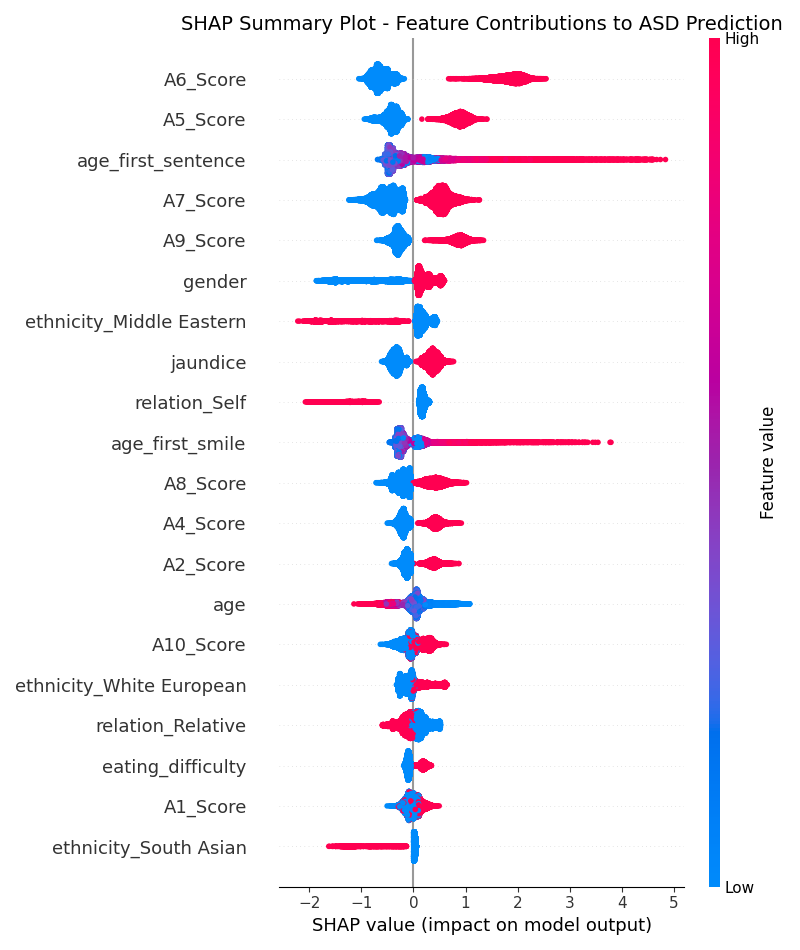
\includegraphics[width=\linewidth]{shap_summary_plot.png}
\end{column}
\begin{column}{0.4\textwidth}
\small
\begin{itemize}
    \item One dot = one patient; \hl{colour = feature value} (red high, blue low).
    \item Right of 0 $\Rightarrow$ pushes towards \hl{ASD}.
    \item \hl{High} AQ-10 scores (red, right) raise ASD risk --- clinically sensible.
    \item Late \texttt{age\_first\_sentence} (red) strongly raises risk.
\end{itemize}
\end{column}
\end{columns}
\end{frame}

\begin{frame}{SHAP --- per-patient explanations}
\begin{columns}
\begin{column}{0.5\textwidth}
\centering {\footnotesize\hl{ASD case} \quad $f(x)=5.77$}\\[2pt]
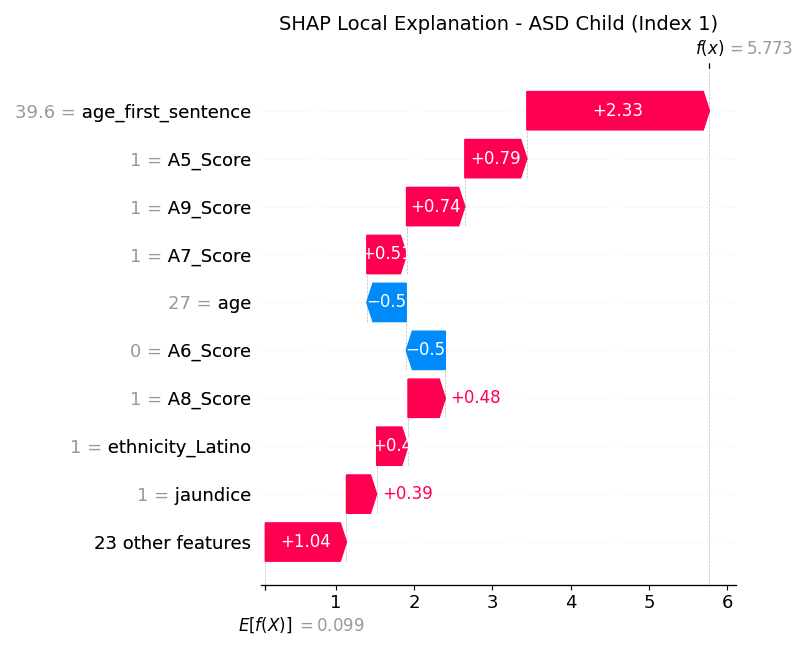
\includegraphics[width=\linewidth]{shap_waterfall_asd.png}
\end{column}
\begin{column}{0.5\textwidth}
\centering {\footnotesize \hl{Non-ASD case} \quad $f(x)=-2.62$}\\[2pt]
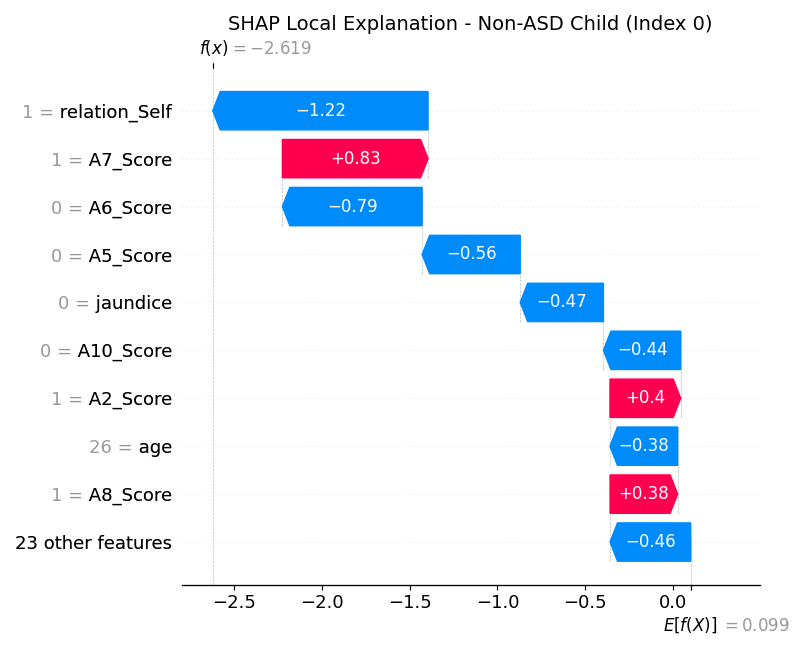
\includegraphics[width=\linewidth]{shap_waterfall_normal.png}
\end{column}
\end{columns}
\vspace{0.1cm}
{\footnotesize \textcolor{accent}{Red} bars push up (towards ASD), blue down. Same model,
a \hl{transparent reason} for every individual prediction.}
\end{frame}

\section{Conclusion}

\begin{frame}{Conclusion \& future work}
\begin{enumerate}
    \item Built a \hl{leakage-free} pipeline --- honest scores over fake-perfect ones.
    \item \hl{GAN/SMOTE} augmentation made the model robust to realistic noise.
    \item Fair race of 10 models: \hl{TabPFN} wins; \hl{stacking} is a steady runner-up.
    \item \hl{SHAP} confirms clinically sensible drivers.
\end{enumerate}
\vspace{0.3cm}
\textbf{Next:} deploy as a phone-based pre-screening aid for parents.
\end{frame}

\section*{References}

\begin{frame}[allowframebreaks]{References}
\footnotesize
\begin{thebibliography}{9}
\bibitem{kaggle} Kaggle, \emph{Autism Prediction Challenge} dataset.
\bibitem{smote} Chawla et al. (2002). \emph{SMOTE: Synthetic Minority Over-sampling Technique}. JAIR.
\bibitem{gan} Goodfellow et al. (2014). \emph{Generative Adversarial Networks}. arXiv:1406.2661.
\bibitem{xgb} Chen \& Guestrin (2016). \emph{XGBoost: A Scalable Tree Boosting System}. arXiv:1603.02754.
\bibitem{lgbm} Ke et al. (2017). \emph{LightGBM: A Highly Efficient Gradient Boosting Decision Tree}. NeurIPS.
\bibitem{catboost} Prokhorenkova et al. (2018). \emph{CatBoost: Unbiased Boosting with Categorical Features}. arXiv:1706.09516.
\bibitem{shap} Lundberg \& Lee (2017). \emph{A Unified Approach to Interpreting Model Predictions (SHAP)}. arXiv:1705.07874.
\bibitem{tabpfn} Hollmann et al. (2022). \emph{TabPFN: A Transformer That Solves Small Tabular Problems in a Second}. arXiv:2207.01848.
\bibitem{tabm} Gorishniy et al. (2024). \emph{TabM: Advancing Tabular DL with Parameter-Efficient Ensembling}. arXiv:2410.24210.
\end{thebibliography}
\end{frame}

\begin{frame}
\begin{center}
{\Large\textbf{\color{accent}Thank you!}}\\[0.4cm]
{\footnotesize Questions \& discussion}
\end{center}
\end{frame}

\end{document}
